
%-----------------------------------------------------------------------------
%	PACKAGES AND THEMES
%-----------------------------------------------------------------------------
\documentclass[ignorenonframetext]{beamer}
\mode<presentation> {
	\usetheme{PrezCMLA}
	\usecolortheme{PrezCMLA}
	\setbeamertemplate{navigation symbols}{} % Remove the navigation symbols
}

\usepackage{graphicx}
\graphicspath{{images/}}
\usepackage{booktabs} % Allows the use of \toprule, \midrule and \bottomrule in tables
\usepackage[utf8]{inputenc}
\usepackage[frenchb]{babel}


\usepackage{tikz}
\usetikzlibrary{shapes,arrows,patterns}


\setbeamertemplate{bibliography item}{}
\setbeamertemplate{bibliography entry title}{}
\setbeamertemplate{bibliography entry location}{}
\setbeamertemplate{bibliography entry note}{}
\bibliographystyle{apalike}


\AtBeginSection[]
{
 \begin{frame}<beamer>
 \frametitle{Plan}
 \tableofcontents[currentsection]
 \end{frame}
}

%-----------------------------------------------------------------------------
%	CUSTOM COMANDS
%-----------------------------------------------------------------------------

\def\keypoint#1{\hfill\textcolor{gray}{#1}}
\def\mycite#1{\keypoint{\cite{#1}}}
\newcommand{\smeq}{\medmuskip=0mu \thickmuskip=0mu \thinmuskip=0mu}

\def\extraLogo{

	\includegraphics[height=\SizeLogoPage]{logo_cognac}
	\hskip2em
	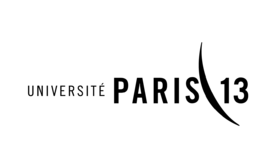
\includegraphics[height=\SizeLogoPage, trim={0 1cm 1cm 1cm}, clip]{logo_UP13}
}


%-----------------------------------------------------------------------------
%	PRESENTATION INFO
%-----------------------------------------------------------------------------

\title[Sparse representation]{Understanding physiological signals via sparse representations}

% Presentation info
\author{Thomas Moreau} % Your name
\institute[CMLA]{ENS Cachan - CMLA} 
\date{15/8/25} % Date, can be changed to a custom date

% Custom footline
\event{MLMDA - Seminar group}
\location{Cachan, FRANCE}

% Add supervisor
\collaborators[collab]{L. Oudre, N. Vayatis}

% Setup the title style
\setbeamertemplate{title page}[frame]
\setlength\SizeTitleBox{.8\textwidth}

%-----------------------------------------------------------------------------
%	DOCUMENT
%-----------------------------------------------------------------------------
\begin{document} 


%% Title page
{\setbeamertemplate{footline}{} 
\begin{frame}[t,plain]

	\titlepage

\end{frame}}


\begin{frame}<beamer>
 \frametitle{Plan}
 \tableofcontents
\end{frame}


\section{Physiological signals}



% Physiological signals ECG
\begin{frame}{Physiological signals}

	\centering
	\Large\textbf{ECG}\\[1em]
	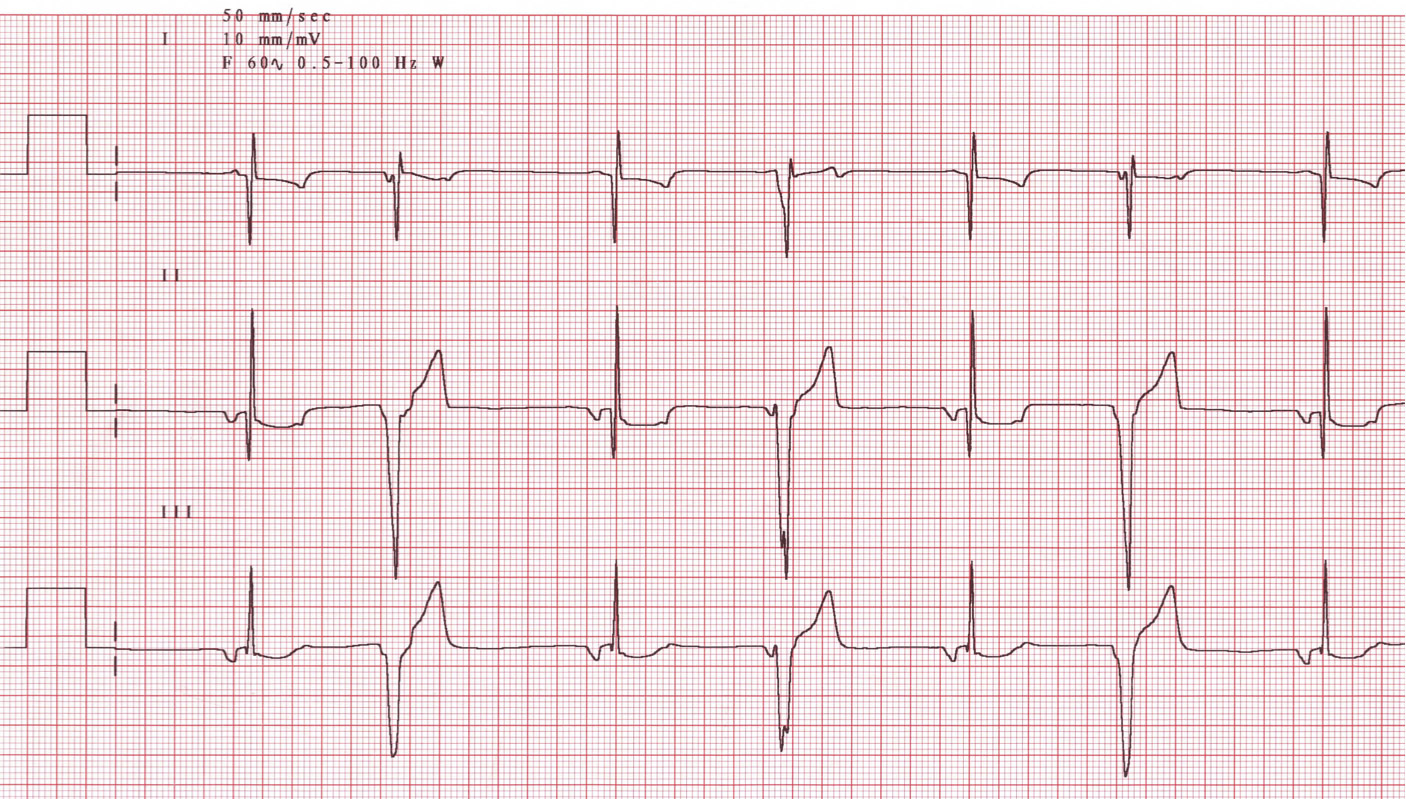
\includegraphics[width=.8\textwidth, height=7em, trim={0 0 0 2em}, clip]{ecg}
	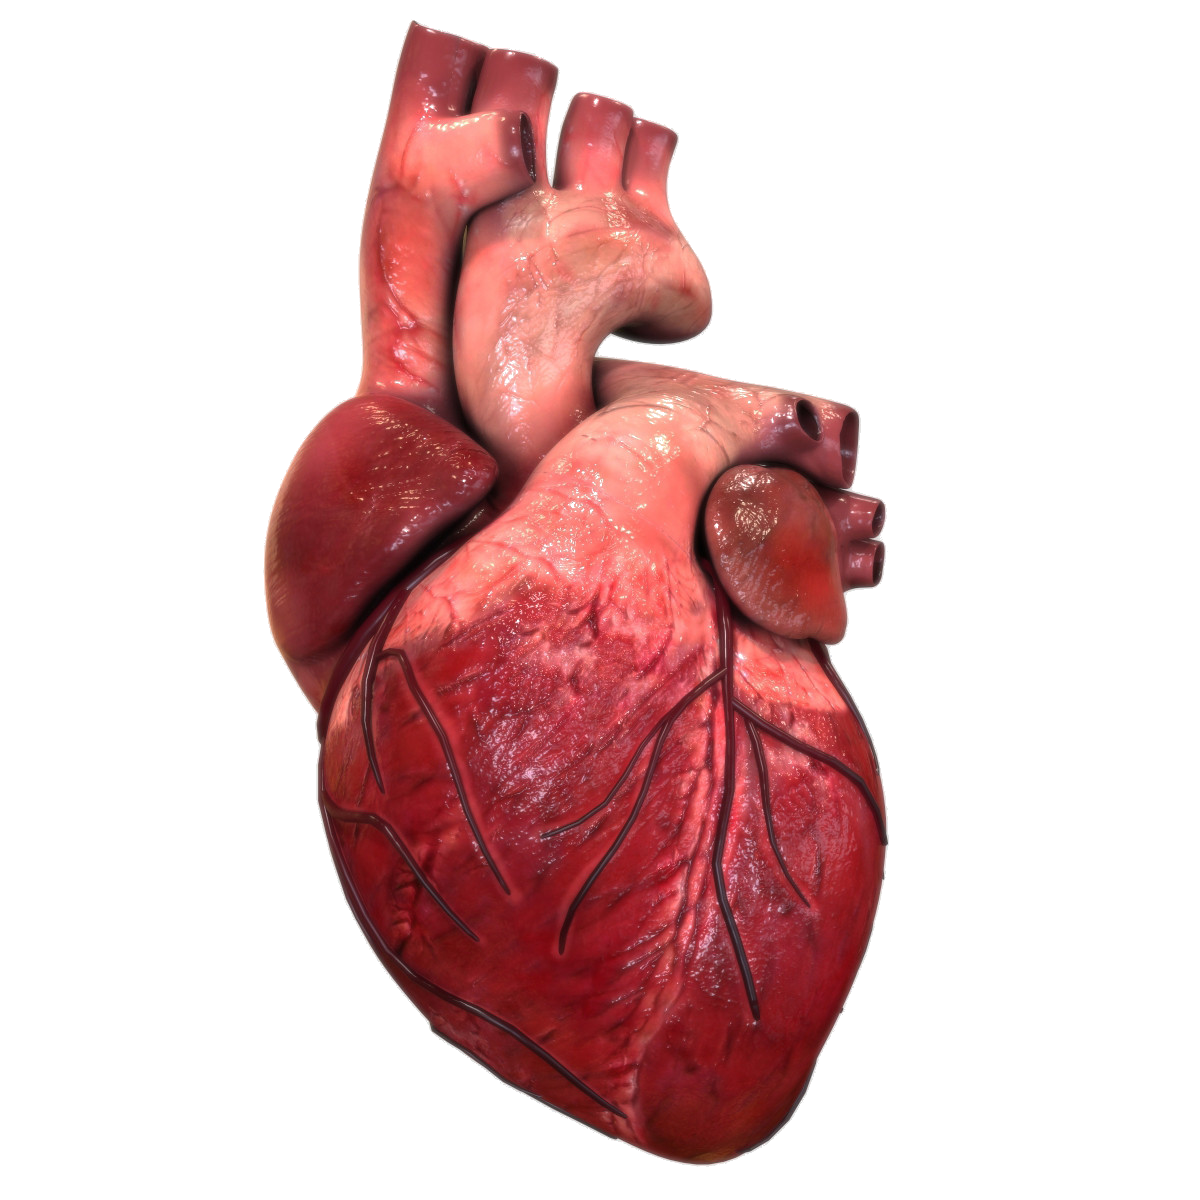
\includegraphics[width=.25\textwidth]{heart}\hskip2em
	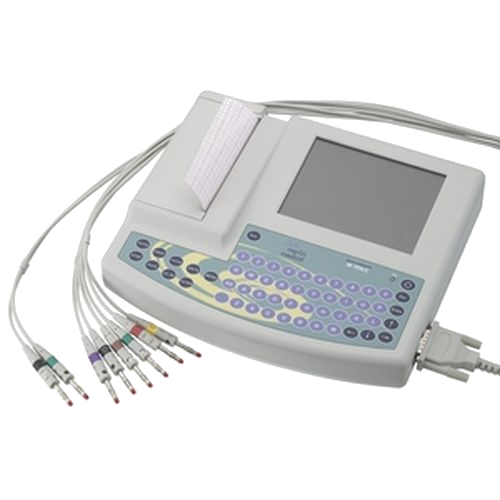
\includegraphics[width=.3\textwidth]{captor_ecg}

\end{frame}


% Physiological signals EEG
\begin{frame}{Physiological signals}

	\centering
	\Large\textbf{EEG}\\[1em]
	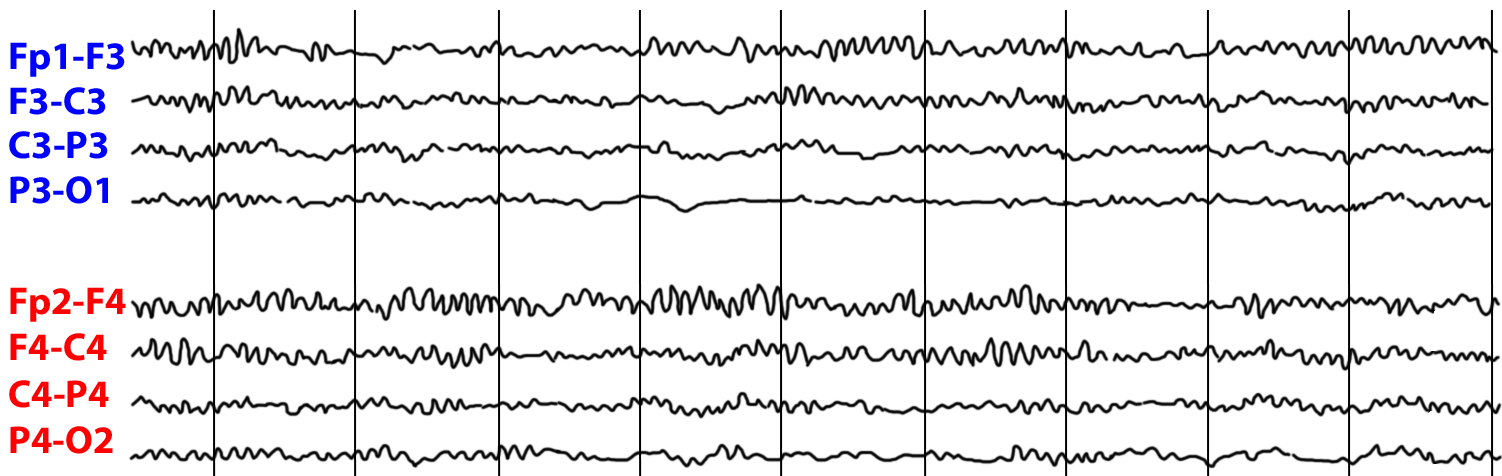
\includegraphics[width=.8\textwidth]{eeg_alpha}\\[.5em]
	
\includegraphics[width=.3\textwidth]{brain}\hskip2em
	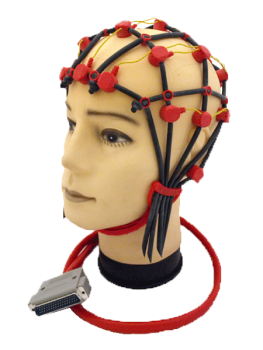
\includegraphics[width=.2\textwidth]{captor_eeg}

\end{frame}






% Physiological signals Oculo
\begin{frame}{Physiological signals}

	\centering
	\Large\textbf{Oculometric signals}\\[.5em]
	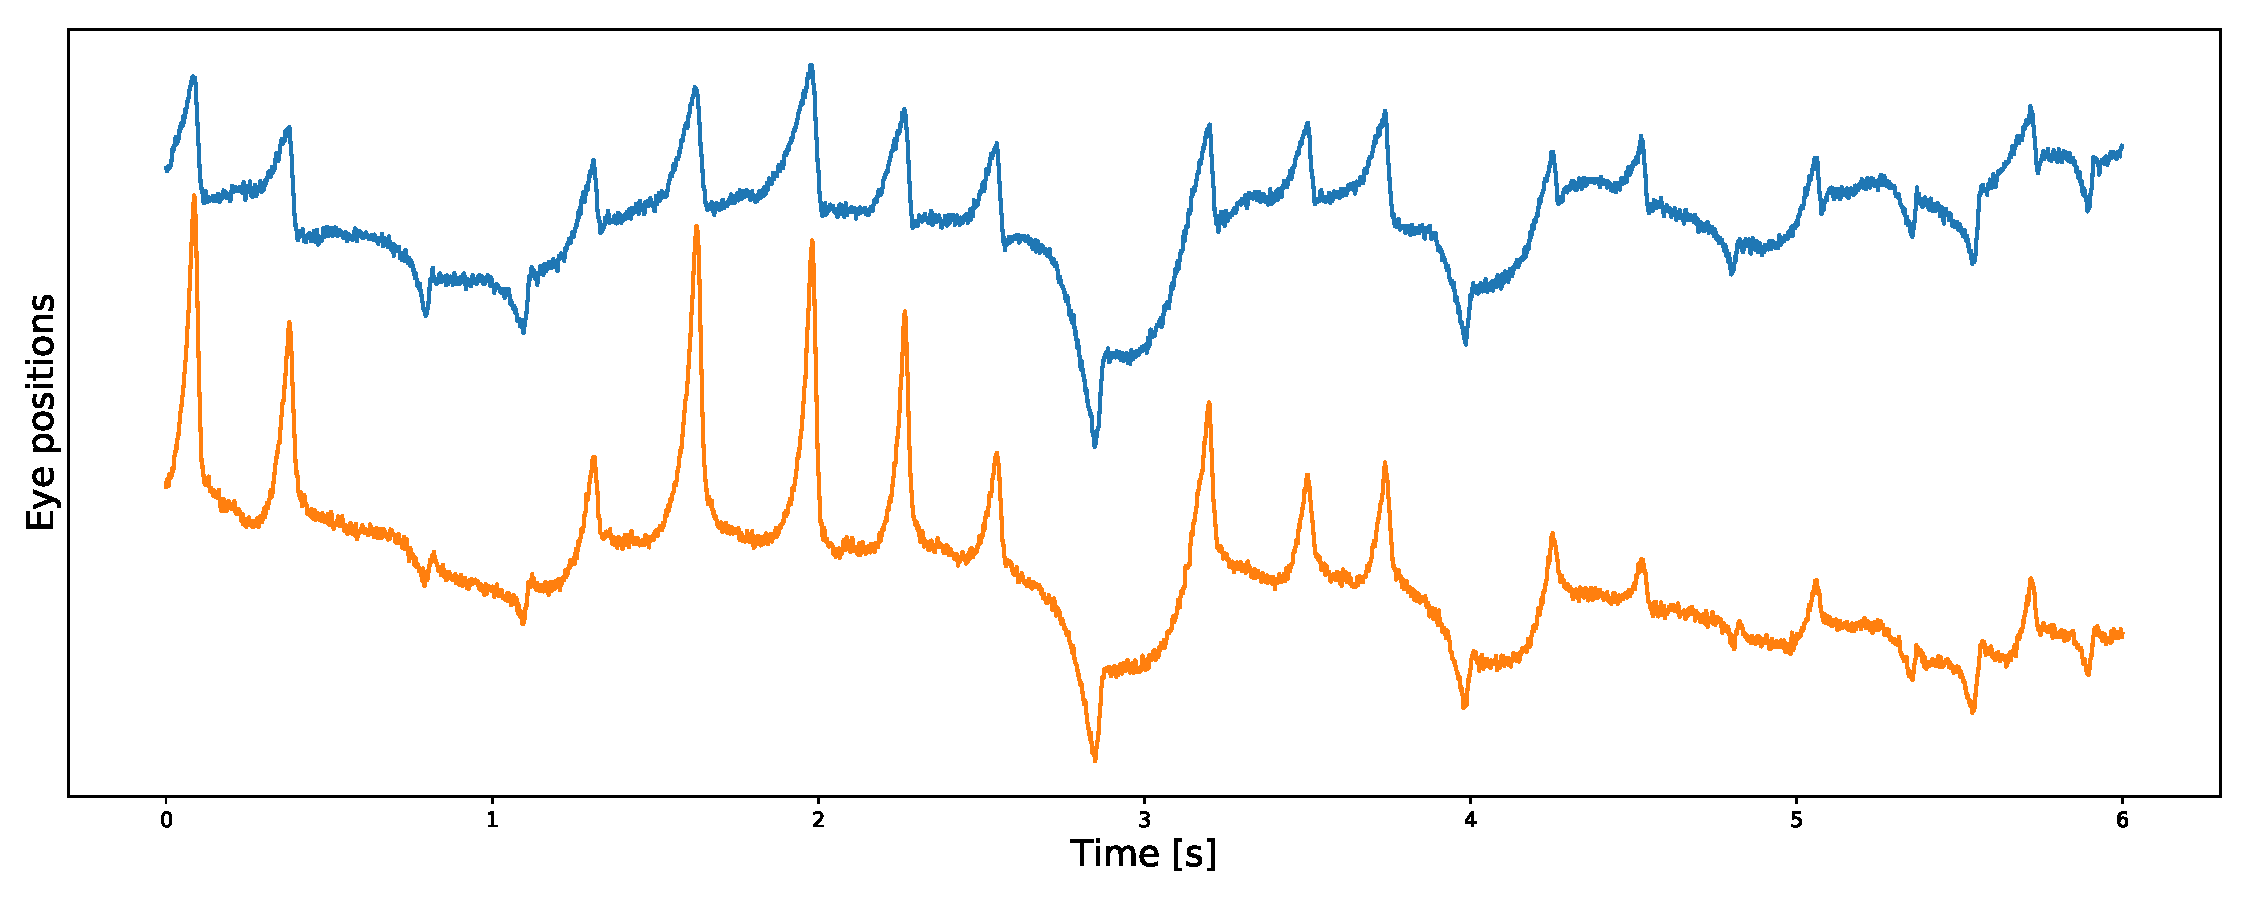
\includegraphics[width=.8\textwidth, height=7em]{oculo}\\[.5em]
	
\includegraphics[width=.25\textwidth]{eye}\hskip2em
	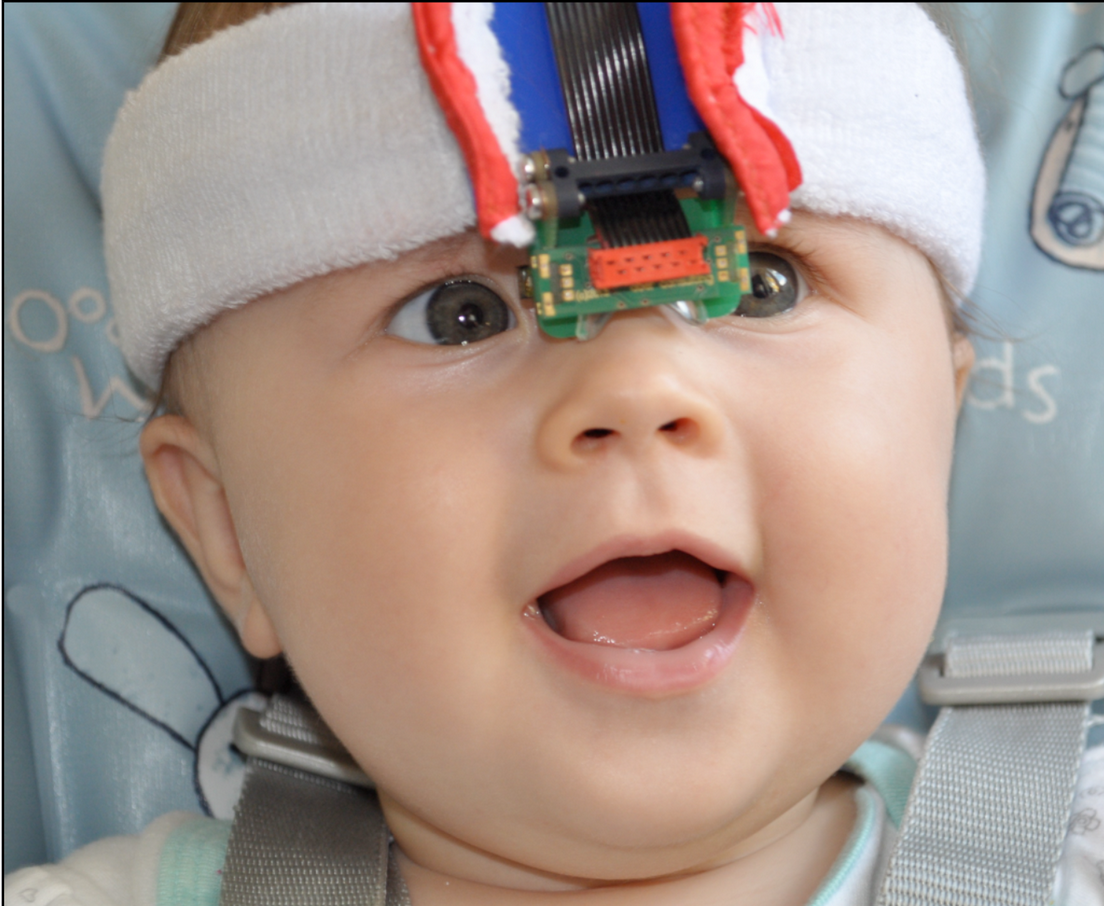
\includegraphics[width=.3\textwidth]{captor_ober}

\end{frame}



% Physiological signals Walk
\begin{frame}{Physiological signals}

	\centering
	\Large\textbf{Accelerometers}\\[1em]
	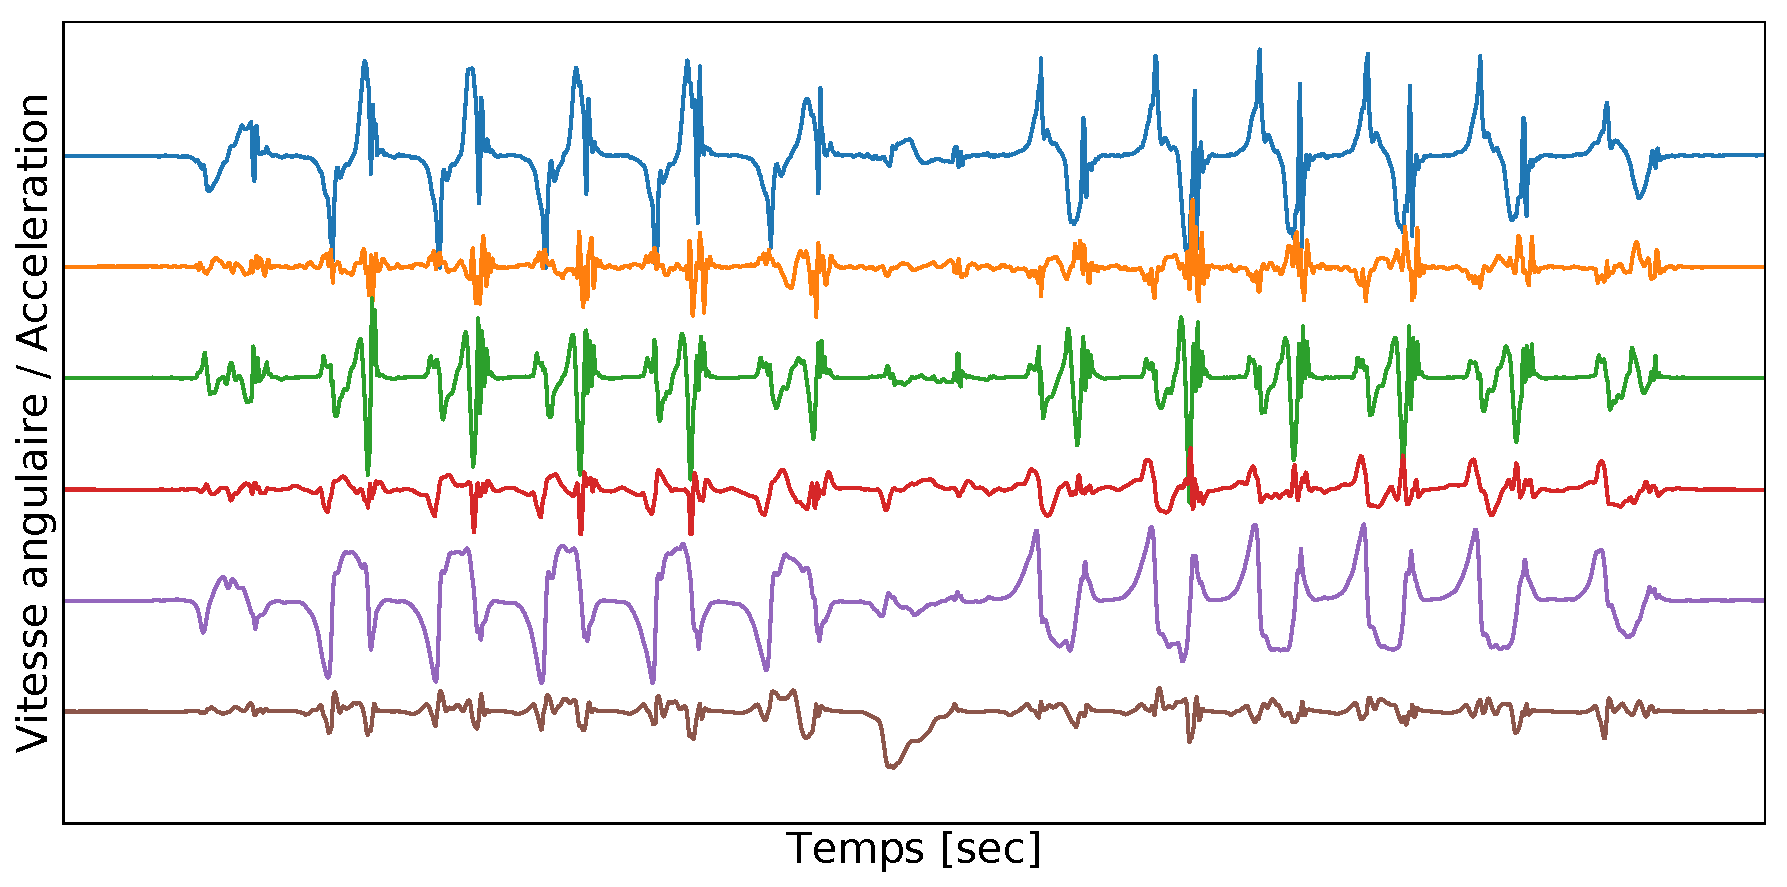
\includegraphics[width=.8\textwidth, height=7em]{accelero}\\[.5em]
	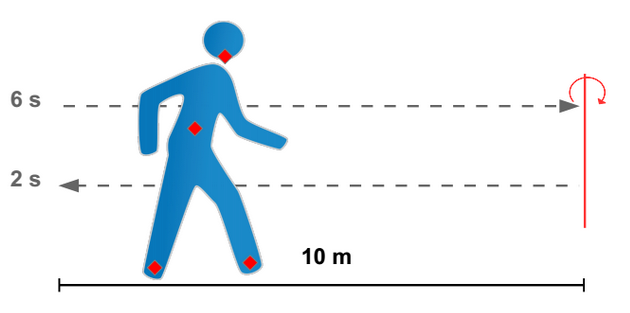
\includegraphics[width=.4\textwidth]{exo_marche}\hskip2em
	\raisebox{2.5em}{\Large $4\times$} 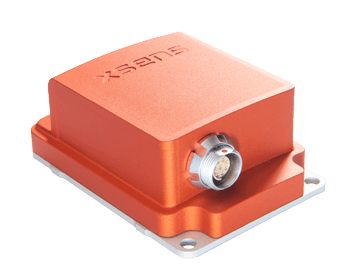
\includegraphics[width=.3\textwidth]{xsens}

\end{frame}

% Statistical tools for signal analysis
\begin{frame}{Statistical analysis for Time Series}
\setbeamercovered{transparent}
\Large

	\begin{itemize}\itemsep1em
		\item Failure of the vectorial distances\\[.5em]
		\begin{itemize}\itemsep1em\itemindent0em
		\item Alignment issues, different lengths \keypoint{(can be solved with DTW)}
		\item "Curse of dimensionality"
	\end{itemize}
		\item Different approaches which can be classified in 2 categories:\\[.5em]
	\begin{itemize}[<1>]\itemsep1em
		\item <-2>{Model based methods (feature extraction + vectorial method, \dots)} 
		\item Data driven methods (End-to-end model, Neural networks, \dots)
	\end{itemize}
	\end{itemize}

\end{frame}


\section{Time Series Representations}


\begin{frame}{Time series representation}
\Large

	{\bf Finding a good representation is challenging:}\\[.5em]
	\begin{itemize}\itemindent2em\itemsep.25em
		\item Samples with various lengths and scales, \\[.25em]
		\keypoint{Invariant}
		\item Heterogeneous sampling rates across channels, \\[.25em]
		\keypoint{Nonparametric}
		\item Samples have high dimension, \\[.25em]
		\keypoint{Scalable}
		\item Non stationary signals. \\[.25em]
		\keypoint{Robust}
	\end{itemize}

\end{frame}



\begin{frame}{Temporal representation}
\large
	\begin{center}
		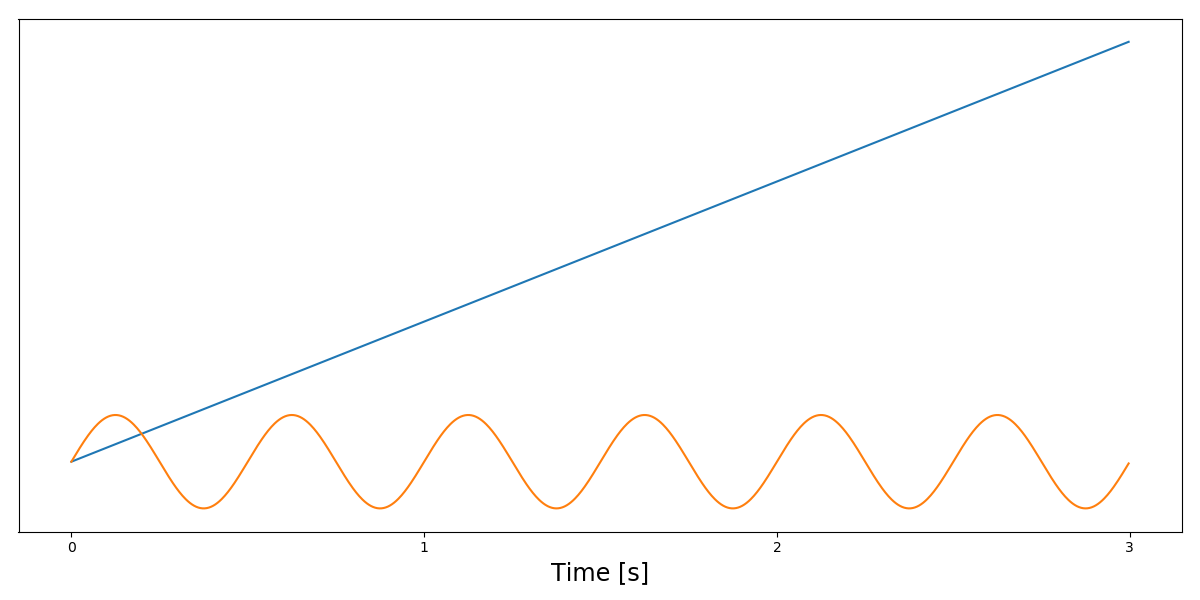
\includegraphics[width=.9\textwidth]{temporal}
	\end{center}
	\begin{itemize}\itemsep1em
		\item Most common representation \hskip1em {\usebeamercolor[fg]{itemize item}\raisebox{0.12ex}{$\blacktriangleright$}\hskip0.1em} Can be efficient (cardiologist)
		\item Permits to detect patterns (linearity, periodicity, ...)
	\end{itemize}
\end{frame}



\begin{frame}{Temporal representation}
	\begin{columns}[c]
		\column{.02\textwidth}
		\column{.5\textwidth}
		\includegraphics[width=.87\textwidth, trim={0 0 21.5em 0}, clip]{fourier_rpz}
		\column{.39\textwidth}
		{\large
		\begin{itemize}\itemsep2em
			\item Not robust to noise
			\item Limited interpretation
		\end{itemize}
		}
	\end{columns}
	
\end{frame}

\begin{frame}{Fourier representation}
	\begin{center}
		%\includegraphics[width=.87\textwidth]{fourier_rpz}
        \begin{tikzpicture}
            \node[anchor=south west,inner sep=0] (image) at (0,0) {\includegraphics[width=.87\textwidth]{fourier_rpz}};
            \node[align=center,font={\Large\bfseries}, rotate=90, above] at (image.west) {Temporal};
            \node[align=center,font={\Large\bfseries}, rotate=-90, above] at (image.east) {Fourier};
        \end{tikzpicture}
	\end{center}
	
\end{frame}



\begin{frame}{Studying the local structure}

	\centering
	{\Large Not so efficient for non stationary signals.\\[1em]}
	\begin{center}
		
        \begin{tikzpicture}
            \node[anchor=south west,inner sep=0] (image) at (0,0) {
            	\includegraphics[width=.87\textwidth, trim={0 15.7em 0 0}, clip]{stft}};
            \node[align=center,font={\Large\bfseries}, rotate=90, above] at (image.west) {Temporal};
            \node[align=center,font={\Large\bfseries}, rotate=-90, above] at (image.east) {Fourier};
        \end{tikzpicture}
	\end{center}

\end{frame}

\begin{frame}{Studying the local structure}

	\centering
	{\Large Need some time-frequency insights.\\[1em]}
	\begin{center}
		\includegraphics[width=.87\textwidth, trim={0 0 0 15.8em}, clip]{stft}
	\end{center}
	
	\Large {\bf Main idea:}\\
	apply global representation to windowed signals

\end{frame}



\begin{frame}{Analytical property}

	\centering \Large
	{\bf Main drawback: }\\[1em]
	We need to know the property we are looking for.\\[2em]
	
	Data-driven representation

\end{frame}





%%%%%%%%%%%%%%%%%%%%%%%%%%%%%%%%%%%%%%%%%%%%%%%%%%%%%%%%%%%%%%%%%%%%%%%%%%%%%%%%
%%%%%%%%%%%%%%%%%%%%%%%%%%%%%%%%%%%%%%%%%%%%%%%%%%%%%%%%%%%%%%%%%%%%%%%%%%%%%%%%
%
%	CSC
%
%%%%%%%%%%%%%%%%%%%%%%%%%%%%%%%%%%%%%%%%%%%%%%%%%%%%%%%%%%%%%%%%%%%%%%%%%%%%%%%%
%%%%%%%%%%%%%%%%%%%%%%%%%%%%%%%%%%%%%%%%%%%%%%%%%%%%%%%%%%%%%%%%%%%%%%%%%%%%%%%%

\section{Singular Spectrum Analysis (SSA)}

\begin{frame}{Singular Spectrum Analysis (SSA) \mycite{Vautard1989}}
\large
	\begin{columns}[T]
		\column{.47\textwidth}
		{\bf Idea}\\[1em]
		\begin{itemize}
			\item Choose a window size $K$ and extract sub series,
			\item Reconstruct a low rank estimate of all the $K$-length sub series,
			\item Decomposition of the series as a sum of "low rank" components.
		\end{itemize}
		\column{.47\textwidth}
		{\usebeamercolor[bg]{itemize}.}\vskip2em
		\begin{itemize}\itemsep1em
		\item[$\rightarrow$] K-trajectory matrix $\pmb X^{(K)}$
		\item[$\rightarrow$] Singular Value decomposition
		$X^{(K)} = \sum_{k=1}^K \lambda_k U_kV_k^T$
		\item[$\rightarrow$] Average along anti-diagonals
	\end{itemize}
	\end{columns}
	\vskip2em
	\begin{columns}[T]
		\column{.9\textwidth}
	
		\begin{itemize}
			\item[$\Rightarrow$] Extract components linked to trend and oscillations
			%\hskip-2em{\bf Issues}
			%\item[$\bullet$] Same pattern present in different low rank components
			%\item[$\bullet$] Representation is "dense", no localization
		\end{itemize}
	
	\end{columns}
\end{frame}



\begin{frame}{Singular Spectrum Analysis}
\large
	In practice, this solves the following problem

\vskip.6em
\begin{block}{Optimization problem}
Solve a convolutional list square
\begin{equation}\label{eq:sparse_code}
	Z^*, \pmb D^* = \arg\min_{Z, \pmb D} \frac{1}{2} \left\|X - \sum_{k=1}^K z_k*D_k\right\|_2^2,
\end{equation}
with constraints $\langle D_i, D_j \rangle = \delta_{i, j}$ 
\end{block}

\vskip1em
\begin{itemize}
	\item $\pmb D$ is the dictionary with $K$ patterns in $\mathbb R$ of length $W$
	\item $Z$ is an activation signal, or coding signal in $\mathbb R^K$ of length $L = T-W+1$
\end{itemize}
\end{frame}



\begin{frame}{Toward a sparse representation}
\Large
	{\bf Issues}\\[1em]
	\begin{itemize}\itemsep1em
	\item[] Same pattern present in different low rank components
	\item[] Representation is "dense", no localization
	\item[] Different representation for each signal
	\end{itemize}

\end{frame}



%-----------------------------------------------------------------------------

%-----------------------------------------------------------------------------
\section{Convolutional Dictionary Learning}


\begin{frame}{Motivation}

	\centering
	\includegraphics[width=.9\textwidth]{CSC}

\end{frame}


\begin{frame}{Dictionary Learning for Time Series}

	\Large
	{\bf Convolutional dictionary learning}\\[2em]

	\begin{itemize}\itemindent2em\itemsep1em
		\item Shift invariant patterns
		\item Separation between the localization and the\\
		\hskip2em shapes of the patterns
	\end{itemize}
\end{frame}


\begin{frame}{Convolutional Sparse Coding}

	For a signal $X$, find the coding signal $Z$ given a set of $K$ patterns $\pmb D$.

	\vskip.6em
	\begin{block}{Optimization problem}
	Solve a $\ell_1$-regularized minimization problem
	\begin{equation}\label{eq:sparse_code}
		Z^* = \arg\min_{z} E(z) = \frac{1}{2} \|X - \sum_{k=1}^Kz_k*\pmb D_k\|_2^2 + \lambda\|Z\|_1,
	\end{equation}
	\end{block}

	\vskip.5em
	Existing algorithms do not scale well with the size of the signal $X$.\\[1em]

	\begin{itemize}\itemindent1em
		\item Feature Sign Search (FSS) \mycite{Grosse2007}
		\item Fast Iterative Soft Thresholding (FISTA) \mycite{Chalasani2013}
		\item Fast Convolutional Sparse Coding (FCSC) \mycite{Bristow2013}
		\item Coordinate Descent (CD)  \mycite{Kavukcuoglu2013}
	\end{itemize}

\end{frame}

\begin{frame}{Coordinate Descent (CD)}

Update the problem for one coordinate at each iteration.\\
The problem in one coordinate is:
$$
	e_{k, t}(y) = \frac{\|\pmb D_k\|_2^2}{2}\left(y - \beta_k[t]\right)^2 + \lambda |y|
$$
with {\small $\beta_k[t] = \left(\left(X- \Phi_{k, t}(Z)*\pmb D^T\right)* \widetilde {\pmb D}_k\right)[t]$}.\\[.5em]
Three algorithms based on this idea:\\[.5em]
\begin{itemize}\itemindent2em
	\item Cyclic updates \mycite{Friedman2007}
	\item Random updates \mycite{Nesterov2010}
	\item Greedy updates \mycite{Osher2009}
\end{itemize}
\vskip1em
Recent work shows it is more efficient to use greedy updates.\\\mycite{Nutini}

\end{frame}


\begin{frame}{Convolutional Coordinate Descent}

For convolutional CD, we can use greedy updates:
$$
	z'_k = \frac{1}{\|\pmb D_k\|_2^2}\text{Sh}(\beta_k, \lambda),
$$
with {\small $\text{Sh}(y, \lambda) = \text{sign}(y)(|y| - \lambda)_+$}.\\[2em]
This can be done efficiently for this problem  by maintaining $\beta$, with $\mathcal O(KS)$ operations. 	\mycite{Kavukcuoglu2013}

$$
\beta_k^{(q+1)}[t] = \beta_k^{(q)}[t] - \mathcal S_{k, k_0}[t-t_0] (z_{k_0}[t_0]-z'_{k_0}[t_0]),
$$\\[1em]
with $\smeq\mathcal S_{k, k_0}[t] = \sum_{\tau=0}^{S-1}\pmb D_{k}[t+\tau] \pmb D_{k_0}^T[\tau] $.\\[1em]
\end{frame}


\begin{frame}{Improving Convolutional Coordinate Descent(1/2)}

This is not so efficient to only change one coordinate as updates only affect a small range of coefficients.\\[.5em]
We could update $M$ coefficients that are in disjoint neighborhoods in {\bf parallel}.\\[1.5em]

{\bf Issue: }Choose disjoint coordinates\\
Split the signal in $M$ continuous chunks and perform updates:\\[.5em]
\begin{itemize}\itemindent4em\itemsep.5em
	\item Use a lock to avoid updates that are too close,
	\item Use a parameter server to reject multiple updates.
\end{itemize}
\mycite{Scherrer2012, Bradley2011}
\\\mycite{Yu2012, Low2012}

\vskip1.5em
{\bf Is it necessary?}
\end{frame}

\begin{frame}{Improving Convolutional Coordinate Descent (2/2)}

	Consider the cost function $E(z) = \frac{1}{2}\|X - \sum_{k=1}^Kz_k*\pmb D_k\|_2^2 + \lambda\|z\|_1$\\[.5em]

	We denote $\Delta E_0 = E(z^{(q+1)}) - E (z^{(q)})$ the update performed at step $q$ for coefficient $(k_0, t_0)$.\\[1em]
	
If we update simultaneously $(k_0, t_0)$ and $(k_1, t_1)$ coefficients, it can be shown that:
$$
\Delta E_{0, 1} = \underbrace{\Delta E_0 + \Delta E_1}_{\text{iterative steps}} - \underbrace{\mathcal S_{k_0, k_1}[t_1 - t_0] \Delta z_0 \Delta z_1}_{\text{interference}},
$$
\vskip.5em
If interference are not too high, the updates can be asynchronous.
\end{frame}

\begin{frame}{Distributed Convolutional Coordinate Descent (DICOD)}

Each core is responsible for the updates of a chunk of coefficients.\\
\vskip1em
\begin{tikzpicture}
	\pgfmathsetmacro{\iO}{-1.9}
	\pgfmathsetmacro{\ione}{3.6}
	\pgfmathsetmacro{\heighl}{-0.8}
	\pgfmathsetmacro{\heighz}{0.3}
	\pgfmathsetmacro{\sep}{0.05}
	\pgfmathsetmacro{\S}{0.8}
	\pgfmathsetmacro{\r}{(-\iO-1.5)/\S}

	\draw (-5, 1) -- (-1.2, 1) node[midway, above]{$\mathcal C_m$  updated in $(k_0, t_0)$} -- (-1.2, -1.5) -- (-5, -1.5) -- cycle;
	\draw (5, 1) -- (1.2, 1) node[midway, above]{$\mathcal C_{m+1}$ updated in $(k_1, t_1)$} -- (1.2, -1.5) -- (5, -1.5) -- cycle;
	\draw [<-, dashed] (-4.5, 0) -- (-6, 0);
	\draw [<-, dashed] (4.5, 0) -- (6, 0);
	\foreach \s in {-1, 1}
	 \draw[blue] (\s*4.5, \heighl) -- (\s*1.5, \heighl) ;
	\draw[red] (\ione, \heighl) -- ++(0, 0.3) node[above, black] {\tiny$\Delta z_{k_1}[t_1]$};
	\draw[green] (\iO, \heighl) -- ++(0, 0.6)  node[above, black] {\tiny$\Delta z_{k_0}[t_0]$};
	\foreach \x/\y in {2.3/0.3, 1.6/0.1, 2/0.6, 3.1/0.7, 4.2/1, 3.9/0.4, 3.8/-0.1, 3.2/-0.5, \ione/0.1}
		\draw[blue] (\x, \heighl) -- ++(0, \y) ;
	\foreach \x/\y in {2.3/0.56, 2.2/0.2, 2.7/0.5, 3.7/0.4, 4.2/-0.24, 3.9/0.7, 3.8/-0.1, 3.2/0.1, 3.5/-0.4, -\iO/0.2}
		\draw[blue] (-\x, \heighl) -- ++(0, \y);
	\fill[green] (\iO-\S, \heighl-3*\sep) -- ++(0, -\sep) -- ++(\S+\r*\S, 0) -- ++(0, \sep) -- cycle;
	\draw (\iO+\r*\S, \heighl-2*\sep) -- ++(0, -2*\sep) -- ++ (-\r*\S, 0)  -- ++ (0, 0.15) -- ++ (0, -0.15) node [below] {\tiny $t_0$} -- ++(-0.8, 0) node[below, black] {\tiny \smeq$t_0 - S$} -- ++(0, +0.1);

	\fill[green] (1.5, \heighl-3*\sep) -- ++(0, -\sep) -- ++(\S-\r*\S, 0) -- ++(0, \sep) -- cycle;
	\draw (1.5, \heighl-2*\sep) -- ++(0, -0.1) -- ++(\S-\r*\S, 0) node[below, black] {\tiny  \smeq$t_0 + S$} -- ++(0, +0.1);
	\fill[red] (\ione-\S, \heighl-3*\sep) -- ++(0, -\sep) -- ++(2*\S, 0) -- ++(0, \sep) -- cycle;
	\draw (\ione-\S, \heighl-2*\sep) -- ++(0, -2*\sep) node [below] {\tiny \smeq$t_1-S$} -- ++(\S, 0) -- ++(0, 3*\sep)  -- ++(0, -3*\sep) node [below] {\tiny $t_1$}-- ++(\S, 0) node [below] { \smeq \tiny$t_1+S$} -- ++(0, 2*\sep);
	%\draw (-3.5, 1) node[below] {};
	\draw (-4.5, \heighl) node[left] {$\beta$};
	\draw (4.5, \heighl) node[right] {$\beta$};

	%% Z on top in green
	 
	\draw[red] (4.5, \heighz) -- (1.5, \heighz) ;
	\foreach \x/\y in {2.3/0.3, 1.6/0.1, 2/0.6, 3.1/0.1, 4.2/0.6, 3.9/0.4, 3.8/-0.1, 3.2/-0.5, \ione/0.3}
		\draw[red] (\x, \heighz) -- ++(0, \y) ;
	\draw[green] (-4.5, \heighz) -- (-1.5, \heighz) ;
	\foreach \x/\y in {2.3/0.56, 2.2/0.2, 2.7/0.5, 3.7/0.4, 4.2/-0.24, 3.9/0.7, 3.8/-0.1, 3.2/0.1, 3.5/-0.4, -\iO/0.6}
		\draw[green] (-\x, \heighz) -- ++(0, \y);
	\draw (-4.5, \heighz) node[left] {$Z$};
	\draw (4.5, \heighz) node[right] {$Z$};


	\draw[-triangle 90] (-1.3, 0) arc (135:40:1.8) node[midway, above] {\small$\smeq\Delta z_{k_0}[t_0]$, $k_0$, $t_0$};% -- ++ (0.1, -0.1);
	\draw[-triangle 90] (1.3, -0.5) arc (135:40:-1.8) node[midway, below] {\small No message};% -- ++ (-0.1, 0.1);
\end{tikzpicture}
\vskip2em
Retrieve the notification when possible to update $\beta$.
\end{frame}

\begin{frame}{Convergence Analysis}
We denote:
$$
C_{k_0k_1}[t_0-t_1]= \frac{\mathcal S_{k_0, k_1}[t_0-t_1]}{\|\pmb D_{k_0}\|_2\|\pmb D_{k_1}\|_2}.
$$
\begin{block}{Theorem}
We consider the following assumptions:\\[.3em]
{\bf H1: }
If for all $k_0, k_1, t_0, t_1$ such that $t_0 - t_1 \neq 0$,  $|C_{k_0k_1}[t_0-t_1]| < 1$.\\[.3em]
{\bf H2: }
If there exist $A \in \mathbb N^*$ such that for all $m \in \left \{ 1, \dots M\right \}$ and $q\in \mathbb N$, $\mathcal C_m$ is updated at least once between iteration $q$ and $q + A$ if the solution is not optimal for all coefficients assigned to $\mathcal C_m$.\\[1em]
Under these assumptions, the DICOD algorithm converges to the optimal solution $z^*$ of \mbox{\autoref{eq:sparse_code}}.
\end{block}

\end{frame}

\begin{frame}{Numerical convergence}
	Artificial problems with $\pmb D$ sinusoidal patterns of size $W=200$ in $\mathbb R^7$,
	$Z$ gaussian bernouilli of length $600W$ and $\epsilon$ a white noise such that:
	$$
		X = \sum_{k=1}^Kz_k*\pmb D_k + \epsilon
	$$
\begin{columns}[T]
	\column{.5\textwidth}
		\centering
		\includegraphics[width=\textwidth]{cost_iter}\\
		\scriptsize Cost as a function of the iterations
	\column{.5\textwidth}
		\centering
		\includegraphics[width=\textwidth]{cost_time}\\
		\scriptsize Cost as a function of the runtime
\end{columns}
\end{frame}

\begin{frame}{Complexity Analysis}
	Computational cost of one update for greedy CD is linear in $\mathcal O(T)$:\\[1em]
	\begin{itemize}\itemindent2em\itemsep.5em
	\item Compute potential updates $z'_k[t]$,
	\item Find $(k_0, t_0) = \arg\min_{k, t} |z'_k[t] - z_k[t]|$.
\end{itemize}
\vskip2em
Computational cost for one update of DICOD is linear in $\mathcal O(\frac{T}{M})$:\\[1em]
\begin{itemize}\itemindent2em\itemsep.5em
	\item Same steps but with a signal of size $\frac{T}{M}$.
\end{itemize}
\end{frame}

\begin{frame}{Speedup}
With an analysis of the interference probability, the convergence rate of DICOD with $M$ cores can be bounded by:
\begin{equation}
	\label{eq:seedup}
	\begin{split}
		\mathbb E[S_{dicod}] & \underset{\phantom{\alpha \to 0}}{\ge} \smeq M^2 ( 1- 2\alpha^2M^2\left(\smeq1 +2\alpha^2M^2\right)^{\frac{M}{2}-1})~,\\
		&\smeq\underset{\alpha \to 0}{\gtrsim} M^2(1-2\alpha^2M^2 + \mathcal O(\alpha^4M^4))~.
	\end{split}
\end{equation}
with $\alpha^2 = \left(\frac{SM}{T}\right)^2$ the probability of interference.\\[.5em]
\begin{itemize}
	\item For $\alpha$ close to 0, the speedup is quadratic.
	\item There is a sharp transition as $\alpha$ grows that degrade the performance of the algorithm.
\end{itemize}
\end{frame}


\begin{frame}{Numerical Speedup}

\centering
		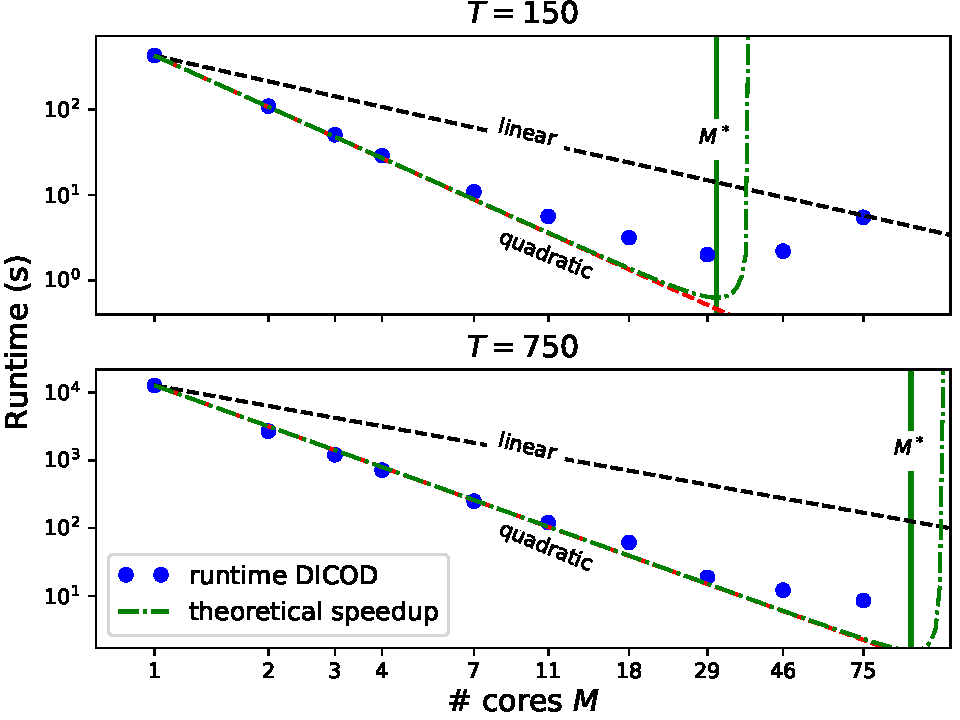
\includegraphics[width=.8\textwidth]{scaling}\\
Runtime as a function of the number of cores

\end{frame}


%--------------------------------------------------------------------------

%--------------------------------------------------------------------------


\begin{frame}{Finishing the process in a linear grid?}
	Non trivial point: {\bf How to decide that the algorithm has converged?}\\[2em]
	
	\begin{itemize}\itemsep2em\itemindent1em
		\item Neighbors paused is not enough!
		\item Define a master 0 and send probes.\\
			\hskip3em Wait for $M$ probes return.
		\item Uses the notion of message queue and network flow.\\
			\hskip3emMaybe we can have better way?
	\end{itemize}
	
	
\end{frame}


\section{Application to physiological signals}


\begin{frame}{Encoding a walk signal}
	\textbf{Protocol:}
	\begin{itemize}\itemsep2em
		\item Select 25 exercises and extract one step from each of them
		\item Encode other exercises using this pattern dictionary.
	\end{itemize}
	\vskip2em
	\textbf{Details:}
	\begin{itemize}
		\item Only used healthy patients in this study,
		\item Use the greedy CD to encode the signals and set $\lambda=5$,
	\end{itemize}

\end{frame}


\begin{frame}{Encoding a walk signal}
	\centering
	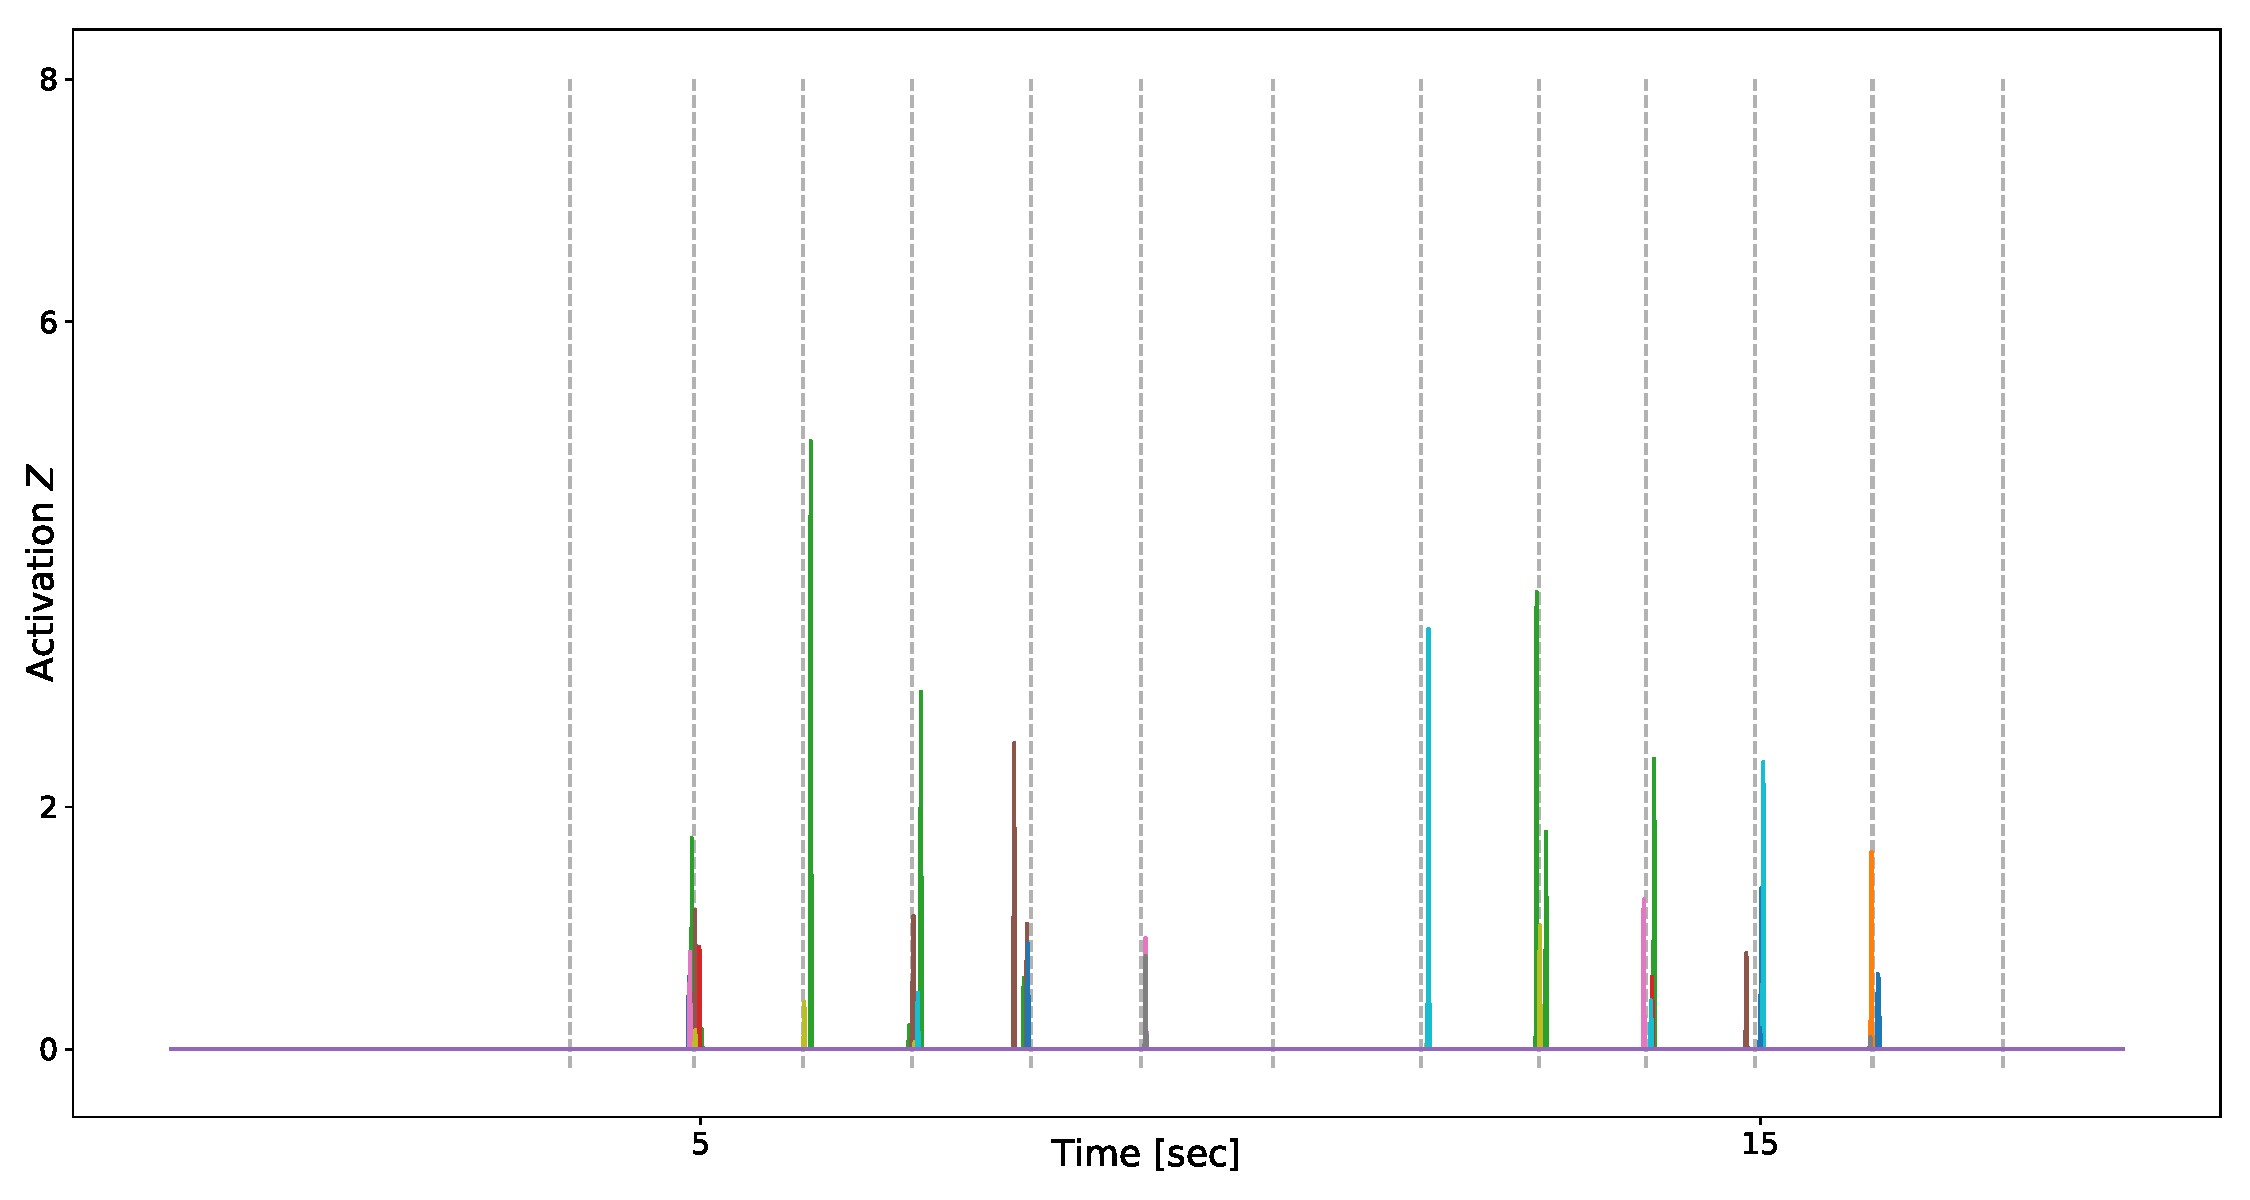
\includegraphics[width=\textwidth]{csc_walk_z}
	The activation are concentrated around the steps but there is some dispersion
	on multiple patterns.
\end{frame}


\begin{frame}{Encoding a walk signal}
	\centering
	\includegraphics[width=\textwidth]{csc_walk_D1}
	Update of the dictionaries with $10$ iterations of alternate minimization and
	FISTA updates for the dictionary.
\end{frame}


\begin{frame}{Encoding a walk signal}
	\centering
	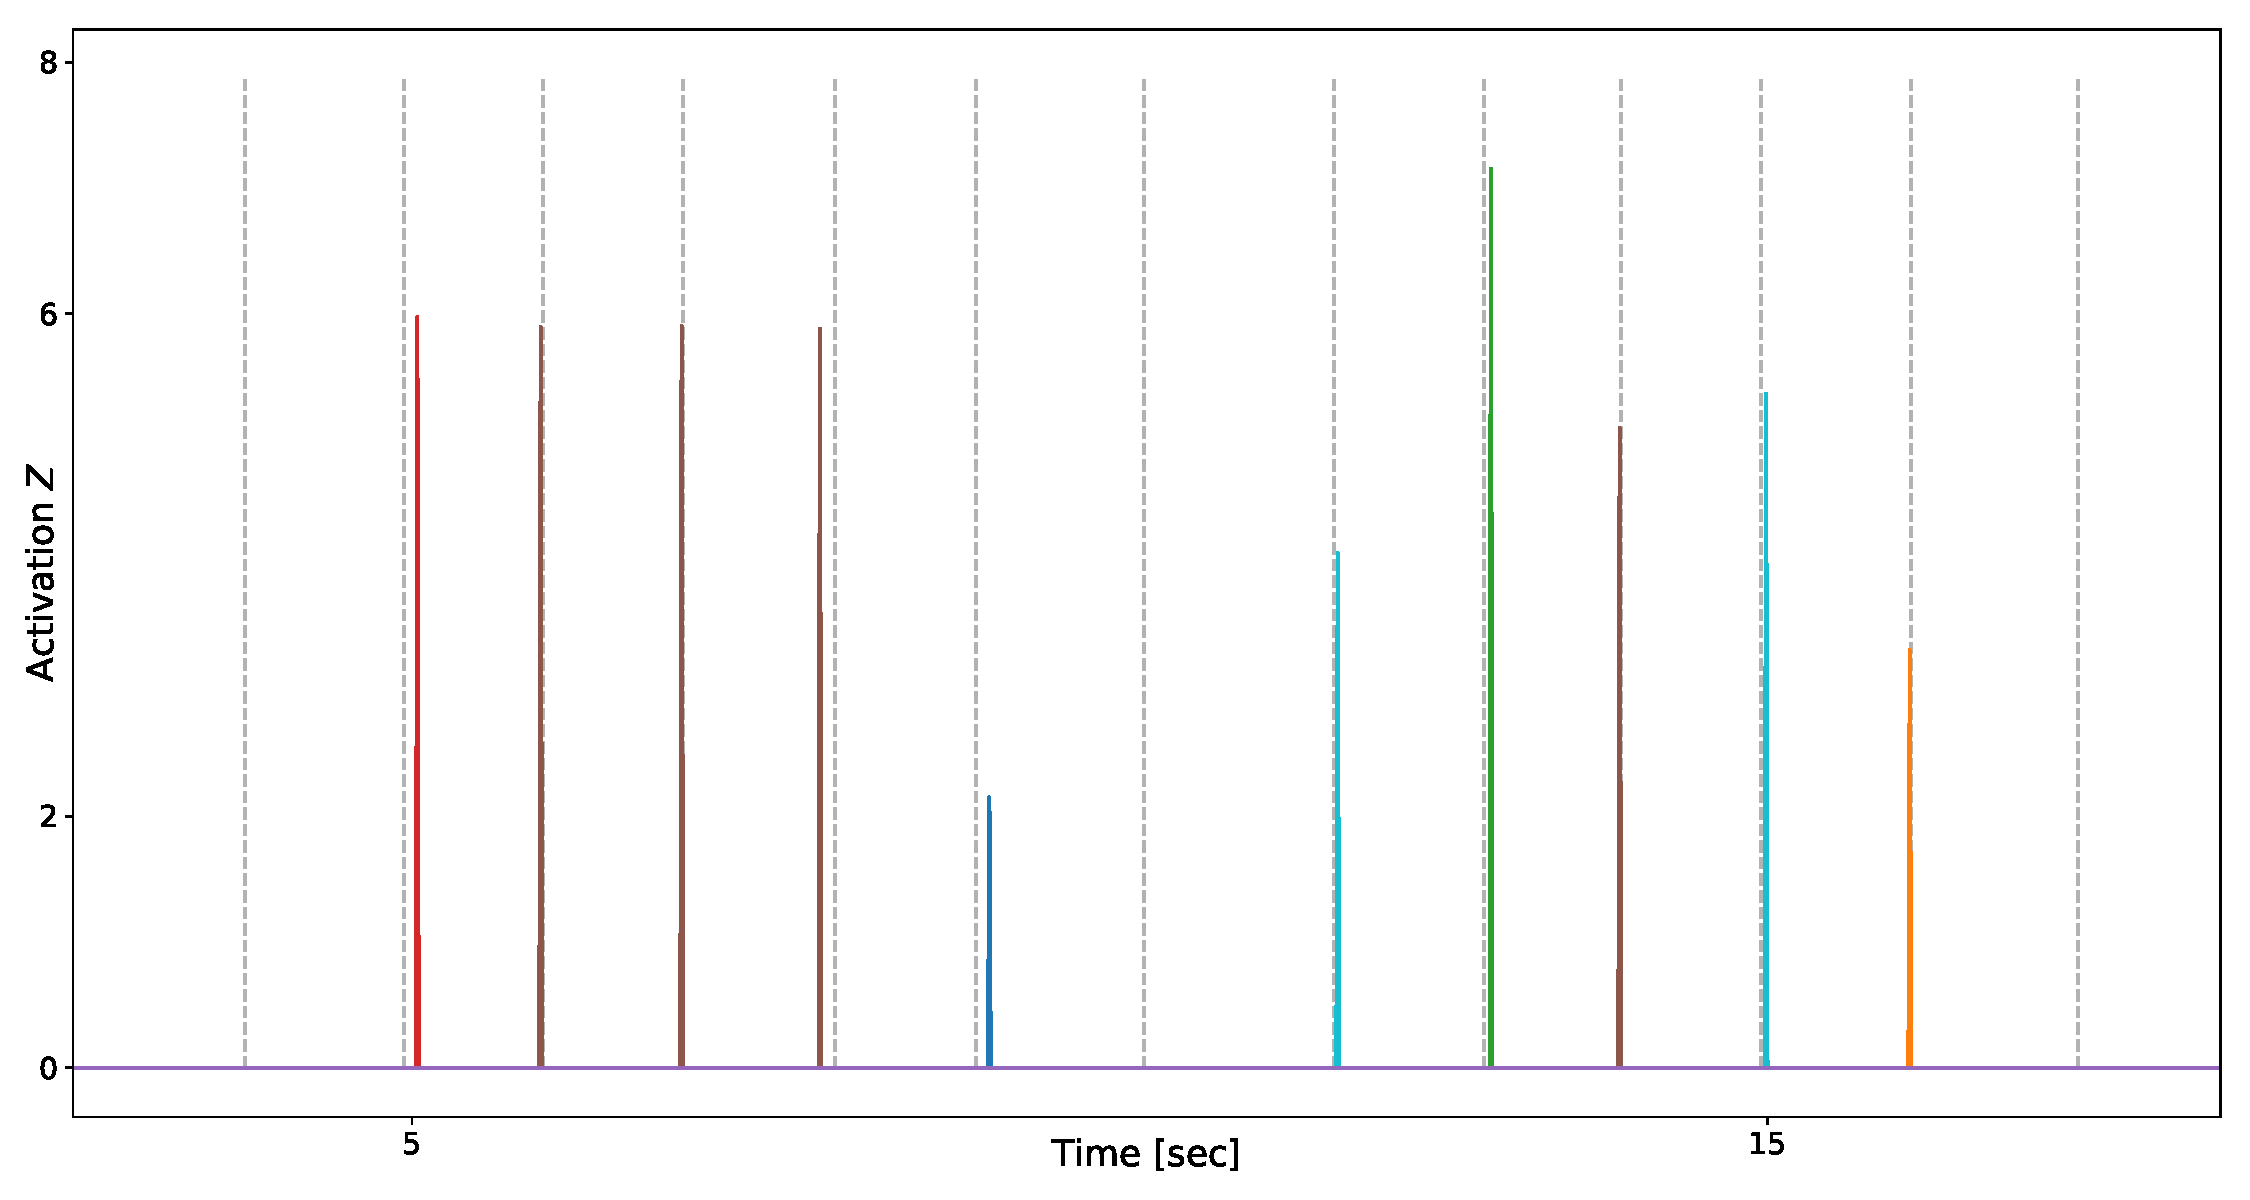
\includegraphics[width=\textwidth]{csc_walk_z1}
	The activation are more concentrated and only activate one pattern.
\end{frame}


\begin{frame}{What next?}
	%TODO Conclusion
	\begin{itemize}\itemsep1em
	\item Find a good way to solve the dictionary learning problem,
	\item Change the penalization? (group sparse),
	\item Use the learned dictionary to extract meaningful features.
\end{itemize}
\end{frame}


	

%-----------------------------------------------------------------------------
% References
%-----------------------------------------------------------------------------
{
\setbeamertemplate{footline}{} 
\begin{frame}{References}
	%\nocite{*}
	\tiny \bibliography{library.bib}
\end{frame}
}

\end{document} 